% Chapter: Analysis & Results — H1: Agenda Distortion

This chapter presents the results of the first hypothesis test. We investigate whether German alternative media outlets systematically diverge from the mainstream news agenda, both in the breadth of topics they cover and in which topics they prioritize. The analysis proceeds in four stages: we first describe the construction and validation of the unified topic space, then present aggregate distortion metrics for each outlet, followed by topic-level statistical tests of over- and under-representation, and finally examine the temporal stability of the observed patterns.

\subsection{Unified Topic Space}

To compare topic coverage across outlets of vastly different sizes---from Anti-Spiegel with 565 articles to Tagesschau with 6,272---we constructed a unified topic space using a merged BERTopic approach. Rather than fitting a single global topic model on the combined corpus, which would allow large outlets to dominate topic discovery, we trained seven independent BERTopic models, one per outlet, each tuned to its respective corpus size. These per-outlet models were then merged into a shared topic space using BERTopic's merge functionality with a cosine similarity threshold of 0.7 \parencite{grootendorst2022bertopic}. This approach ensures that topics relevant to small outlets---which a global model might absorb into noise---are preserved in the unified space.

The merged model produced 74 distinct topics across 20,455 articles. To validate this approach against the literature-standard single global model \parencite{jacobi2016quantitative, muller2022rightwing}, we also trained a global BERTopic on the full corpus. The global model discovered 165 topics but assigned 27--41\% of documents to the outlier category (topic $-1$), compared to 0--10\% for the merged model. Despite these structural differences, the outlet-level distortion rankings produced by both approaches were near-identical (Spearman $\rho = 0.943$, $p = 0.005$), confirming that the merged approach captures the same agenda structure while retaining substantially more documents for analysis.

All articles were then projected through the merged model to obtain topic assignments, and per-outlet topic distributions were computed as the proportion of each outlet's articles assigned to each topic. These distributions form the basis for all subsequent analyses.

\subsection{Aggregate Agenda Distortion}

We assessed agenda distortion using five complementary metrics, each grounded in media communication literature. Following the approach of comparing each outlet individually against Tagesschau as a mainstream reference---rather than collapsing all alternative outlets into a single group---each outlet receives its own distortion profile.

\subsubsection{Metrics}

\textit{Normalized Shannon entropy} measures topic concentration: how evenly an outlet distributes its coverage across available topics \parencite{boydstun2014importance}. Values range from 0 (all articles on one topic) to 1 (uniform distribution). Lower entropy indicates a narrower editorial focus.

\textit{Jensen-Shannon divergence} (JSD) quantifies the overall distance between an outlet's topic distribution and Tagesschau's \parencite{dimaggio2013exploiting}. JSD is symmetric, bounded between 0 and 1, and avoids the asymmetry and unboundedness problems of KL divergence. We use the unweighted variant as recommended by \textcite{gallagher2020divergent}.

\textit{Spearman rank correlation} captures whether outlets prioritize topics in the same order as Tagesschau \parencite{mccombs1972agenda}. A rank-based measure, it is entirely size-independent. Values near $+1$ indicate identical priority orderings; values near $0$ indicate independent agendas.

\textit{Top-K overlap} measures the fraction of an outlet's ten most-covered topics that also appear in Tagesschau's top ten \parencite{heidenreich2020media}. This captures whether the most salient issues align between outlets.

\textit{Coverage breadth} controls for corpus size by comparing the number of topics an outlet covers against the number expected under a binomial model given its size. Values below 1.0 indicate narrower coverage than corpus size would predict.

\subsubsection{Results}

Table~\ref{tab:h1_metrics} reports all five metrics for each outlet. Figure~\ref{fig:h1_metrics_panel} visualises the results.

\begin{table}[H]
\centering
\caption{H1 agenda distortion metrics per outlet (vs Tagesschau)}
\label{tab:h1_metrics}
\begin{tabular}{llrrrrr}
\hline
\textbf{Outlet} & \textbf{Category} & \textbf{Articles} & \textbf{Entropy} & \textbf{JSD} & \textbf{Spearman $\rho$} & \textbf{Top-K} \\
\hline
Tagesschau        & Mainstream       & 6,272 & 0.930 & 0.000 & +1.000 & 1.00 \\
RT DE             & Pro-Russian      & 4,556 & 0.823 & 0.154 & +0.567 & 0.60 \\
Tichys Einblick   & Right-Populist   & 2,756 & 0.903 & 0.148 & +0.460 & 0.30 \\
NIUS              & Right-Populist   & 3,266 & 0.880 & 0.192 & +0.308 & 0.40 \\
Compact           & Right-Wing       & 1,580 & 0.878 & 0.213 & +0.253 & 0.50 \\
Deutschland-Kurier & Right-Wing      & 1,460 & 0.845 & 0.219 & +0.437 & 0.40 \\
Anti-Spiegel      & Pro-Russian      & 565   & 0.734 & 0.398 & +0.347 & 0.40 \\
\hline
\end{tabular}
\end{table}

\begin{figure}[H]
    \centering
    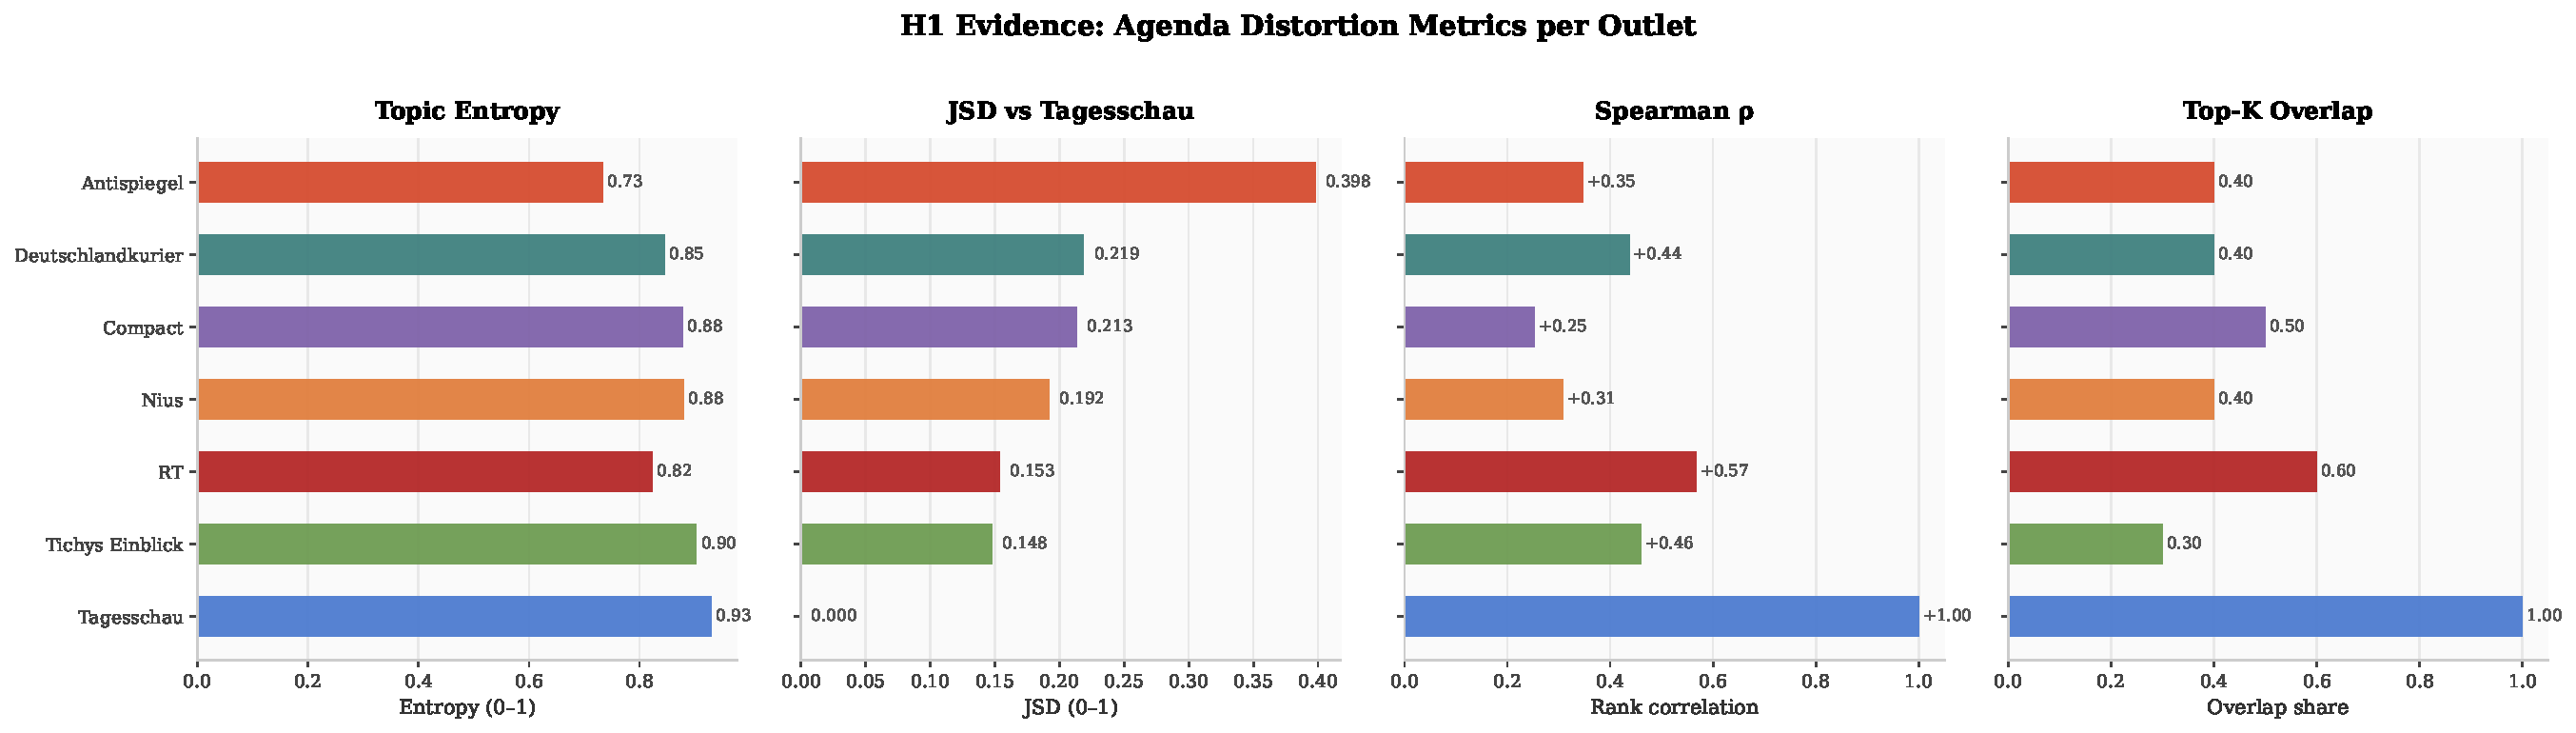
\includegraphics[width=\textwidth]{Images/h1/h1_01_metrics_panel.pdf}
    \caption{Agenda distortion metrics per outlet. From left to right: normalised Shannon entropy (topic concentration), Jensen-Shannon divergence vs Tagesschau (agenda distance), Spearman rank correlation (priority ordering similarity), and top-K topic overlap. All alternative outlets show statistically significant divergence from the mainstream reference.}
    \label{fig:h1_metrics_panel}
\end{figure}

All six alternative outlets diverge significantly from Tagesschau across all metrics. The distortion follows a clear gradient by outlet category. Anti-Spiegel exhibits the strongest distortion on every measure: lowest entropy (0.734), highest JSD (0.398), and narrowest coverage breadth (0.657). At the other end, RT DE and Tichys Einblick show the mildest distortion, though both remain significantly different from the mainstream baseline.

Spearman correlations are positive but moderate across all outlets (0.25--0.57), indicating that alternative outlets do not invert the mainstream agenda but rather shift emphasis. They cover many of the same topics as Tagesschau, but in systematically different proportions. Top-K overlap is uniformly low (0.30--0.60), meaning that at most six of an outlet's ten most-covered topics appear among Tagesschau's top ten.

A particularly instructive case is Tichys Einblick, which has the broadest coverage of any outlet (breadth = 0.925, exceeding Tagesschau's 0.898) yet the lowest top-K overlap (0.30). This outlet covers \textit{more} topics than expected for its size, but emphasises entirely different ones---a pattern consistent with pure agenda-setting in the sense of \textcite{mccombs1972agenda}.

Bootstrap confidence intervals (Figure~\ref{fig:h1_bootstrap_jsd}, $n = 500$ resamples) confirm that all JSD values are significantly above zero, with tight intervals that do not overlap between Anti-Spiegel and the remaining outlets. The JSD confidence intervals for RT DE and Tichys Einblick overlap, meaning these two outlets cannot be statistically distinguished in terms of aggregate agenda distance.

\begin{figure}[H]
    \centering
    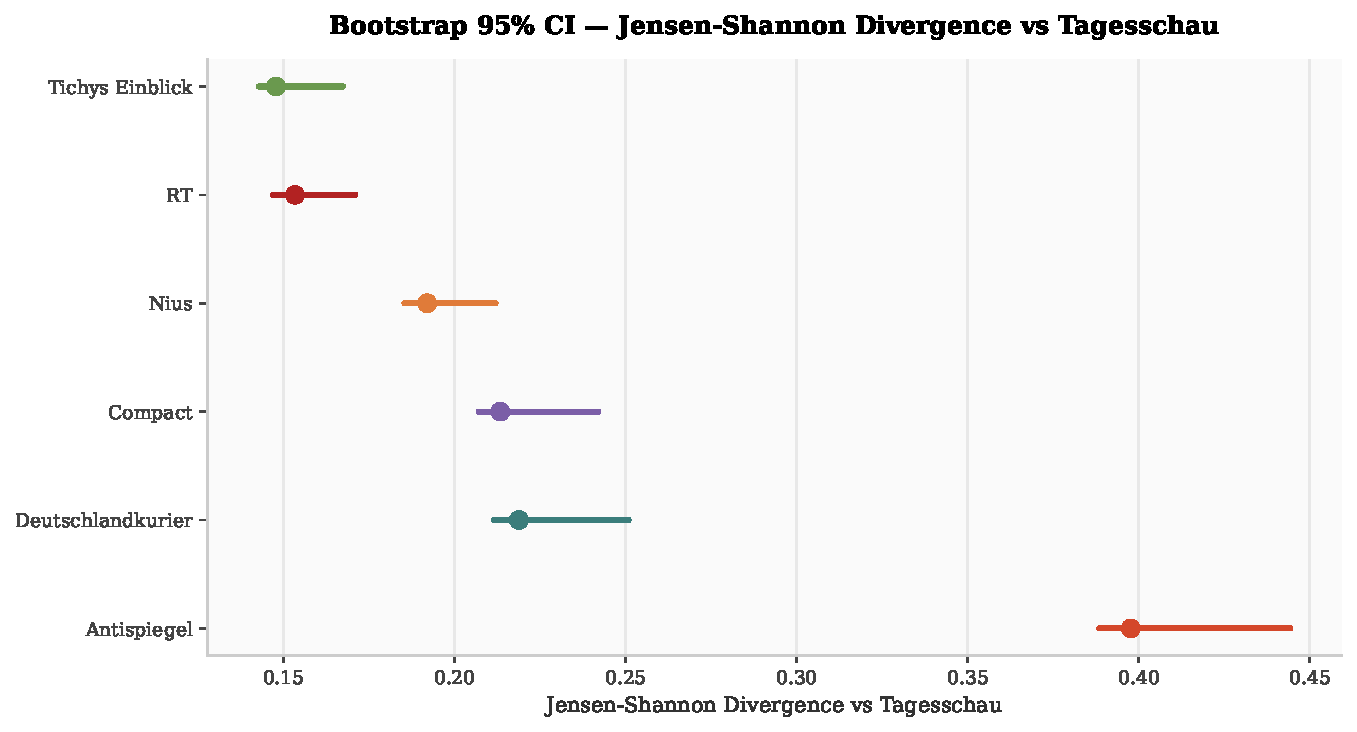
\includegraphics[width=0.85\textwidth]{Images/h1/h1_03_bootstrap_jsd_vs_tagesschau.pdf}
    \caption{Bootstrap 95\% confidence intervals for Jensen-Shannon divergence vs Tagesschau ($n = 500$ stratified resamples). All intervals are well above zero. Anti-Spiegel is in a distinct distortion category; RT DE and Tichys Einblick cannot be statistically distinguished.}
    \label{fig:h1_bootstrap_jsd}
\end{figure}

\subsection{Topic-Level Divergence}

Aggregate metrics establish that agenda distortion exists; topic-level analysis reveals \textit{what} drives it. For each combination of outlet and topic, we conducted a $\chi^2$ test comparing observed topic frequency against Tagesschau's baseline, applying Benjamini-Hochberg false discovery rate correction across all 444 tests (6 outlets $\times$ 74 topics).

Of 444 tests, 275 were significant at FDR $< 0.01$, and 143 were both significant and substantive (difference $\geq$ 1 percentage point). This indicates pervasive, not isolated, agenda divergence.

\subsubsection{The Shared Alternative Media Agenda}

Several topics are significantly over-represented in four or more alternative outlets simultaneously, forming what we term the \textit{shared alternative media agenda}---a set of issues that right-wing, right-populist, and in some cases pro-Russian outlets collectively amplify relative to mainstream coverage. Table~\ref{tab:shared_agenda} presents these topics.

\begin{table}[H]
\centering
\caption{Topics significantly over-represented in four or more alternative outlets (FDR $< 0.01$, difference $\geq$ 1pp vs Tagesschau)}
\label{tab:shared_agenda}
\begin{tabular}{lrll}
\hline
\textbf{Topic} & \textbf{Mean $\Delta$pp} & \textbf{Outlets} & \textbf{All $p_{\text{adj}}$} \\
\hline
AfD / BSW / parties            & +5.5 & DK, Compact, NIUS, Tichys   & $< 10^{-17}$ \\
Merz / chancellor race         & +4.7 & DK, Compact, NIUS, Tichys   & $< 10^{-11}$ \\
Social media / youth           & +4.0 & DK, Compact, NIUS, Tichys   & $< 10^{-12}$ \\
Asylum / migration             & +2.2 & DK, Compact, NIUS, Tichys   & $< 10^{-4}$  \\
Courts / criminal cases        & +2.1 & DK, Compact, NIUS, RT       & $< 10^{-4}$  \\
Coalition politics             & +2.0 & DK, Compact, NIUS, Tichys   & $< 10^{-4}$  \\
\hline
\end{tabular}
\end{table}

The domestic political agenda---party politics, the chancellor race, migration, and crime---is systematically amplified across all right-wing and right-populist outlets. This pattern is consistent with agenda-setting theory: these outlets do not simply report differently on a shared set of topics, but make specific political issues \textit{more salient} relative to their overall output \parencite{mccombs1972agenda}.

\subsubsection{The Pro-Russian Signature}

The two pro-Russian outlets exhibit a distinctive topical signature that sets them apart from both mainstream and domestic right-wing media. Anti-Spiegel devotes 49\% of its coverage to Russia/Ukraine-related topics---the Russia/Ukraine conflict from a Russian perspective (+17.5pp vs Tagesschau, $p < 10^{-106}$), Ukraine/Putin/Selenskyj coverage (+12.8pp, $p < 10^{-34}$), and bilateral Russia-Ukraine relations (+9.4pp, $p < 10^{-28}$). RT DE follows a similar pattern at lower intensity, devoting 32\% of coverage to these topics. For comparison, Tagesschau allocates approximately 9\% of its coverage to the same set of topics. This extreme over-representation constitutes the single strongest agenda distortion signal in the dataset.

\subsubsection{Systematic Under-Representation}

All six alternative outlets significantly under-represent financial market coverage (DAX, stocks; all $p < 10^{-9}$) and, to varying degrees, apolitical hard news such as natural disasters, health, and international non-conflict topics. The right-wing and populist-alternative outlets additionally under-represent Israel/Gaza coverage by 2.9--5.8 percentage points relative to Tagesschau ($p < 10^{-10}$). This selective de-prioritisation of apolitical and internationally diverse content reinforces the domestic political focus identified in the over-representation analysis.

\subsection{Outlet Clustering}

To test whether the a priori outlet categorisation (pro-Russian, right-wing, right-populist) is empirically supported by topical similarity, we computed pairwise Jensen-Shannon divergence between all seven outlets and applied hierarchical clustering using Ward's method \parencite{muller2022rightwing}.

\begin{figure}[H]
    \centering
    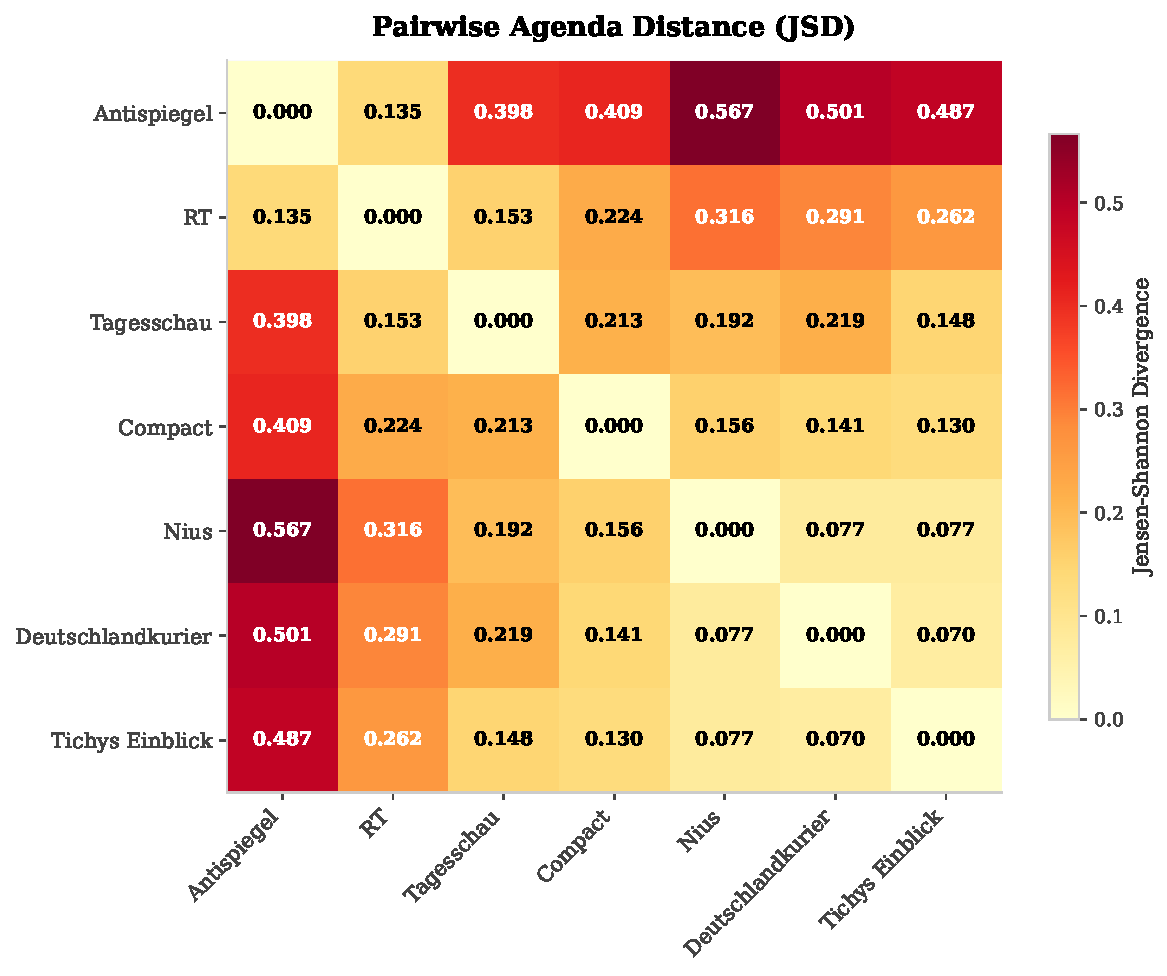
\includegraphics[width=0.85\textwidth]{Images/h1/h1_08_pairwise_jsd_heatmap.pdf}
    \caption{Pairwise Jensen-Shannon divergence between all outlets. Outlets are ordered by hierarchical clustering (Ward's method). The cluster structure mirrors the a priori ideological categorisation.}
    \label{fig:h1_pairwise_jsd}
\end{figure}

\begin{figure}[H]
    \centering
    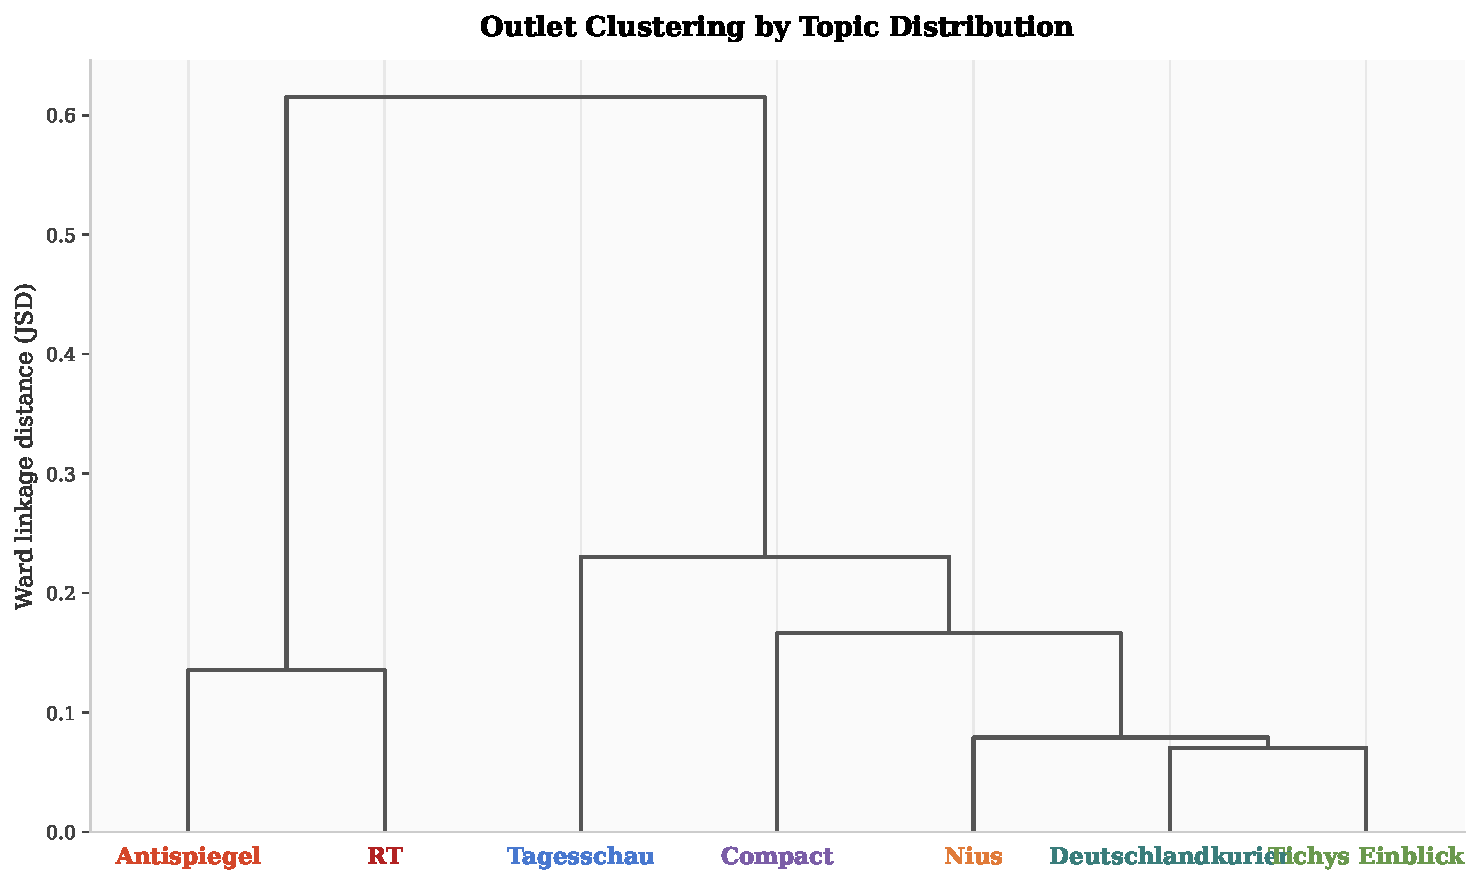
\includegraphics[width=0.85\textwidth]{Images/h1/h1_09_outlet_dendrogram.pdf}
    \caption{Hierarchical clustering dendrogram (Ward's method on pairwise JSD). Three clusters emerge: a domestic right cluster (DK, Tichys, NIUS, Compact), a pro-Russian cluster (RT, Anti-Spiegel), and Tagesschau as isolated mainstream reference.}
    \label{fig:h1_dendrogram}
\end{figure}

The dendrogram (Figure~\ref{fig:h1_dendrogram}) reveals three natural clusters that closely match the a priori categorisation:

\begin{enumerate}
    \item \textbf{Domestic right cluster}: Deutschland-Kurier, Tichys Einblick, NIUS, and Compact form a tight group (pairwise JSD 0.07--0.16). Within this cluster, Deutschland-Kurier and Tichys Einblick are the closest pair (JSD = 0.070), indicating near-identical topic distributions despite their different editorial self-characterisations.
    \item \textbf{Pro-Russian cluster}: Anti-Spiegel and RT DE cluster together (JSD = 0.135), reflecting their shared emphasis on Russia/Ukraine coverage.
    \item \textbf{Mainstream}: Tagesschau stands apart as the most distant outlet from all alternatives (JSD 0.148--0.398).
\end{enumerate}

This empirical clustering validates the outlet categorisation used throughout the analysis and suggests that editorial ideology---rather than outlet size, publication frequency, or other structural factors---is the primary determinant of agenda similarity.

\subsection{Temporal Stability}

Agenda-setting theory is fundamentally concerned with temporal dynamics: who sets the agenda, and does coverage converge or diverge over time \parencite{vargo2017networks}? To address this, we computed rolling Jensen-Shannon divergence using a four-week sliding window across the 27-week study period (August 2025--January 2026).

\begin{figure}[H]
    \centering
    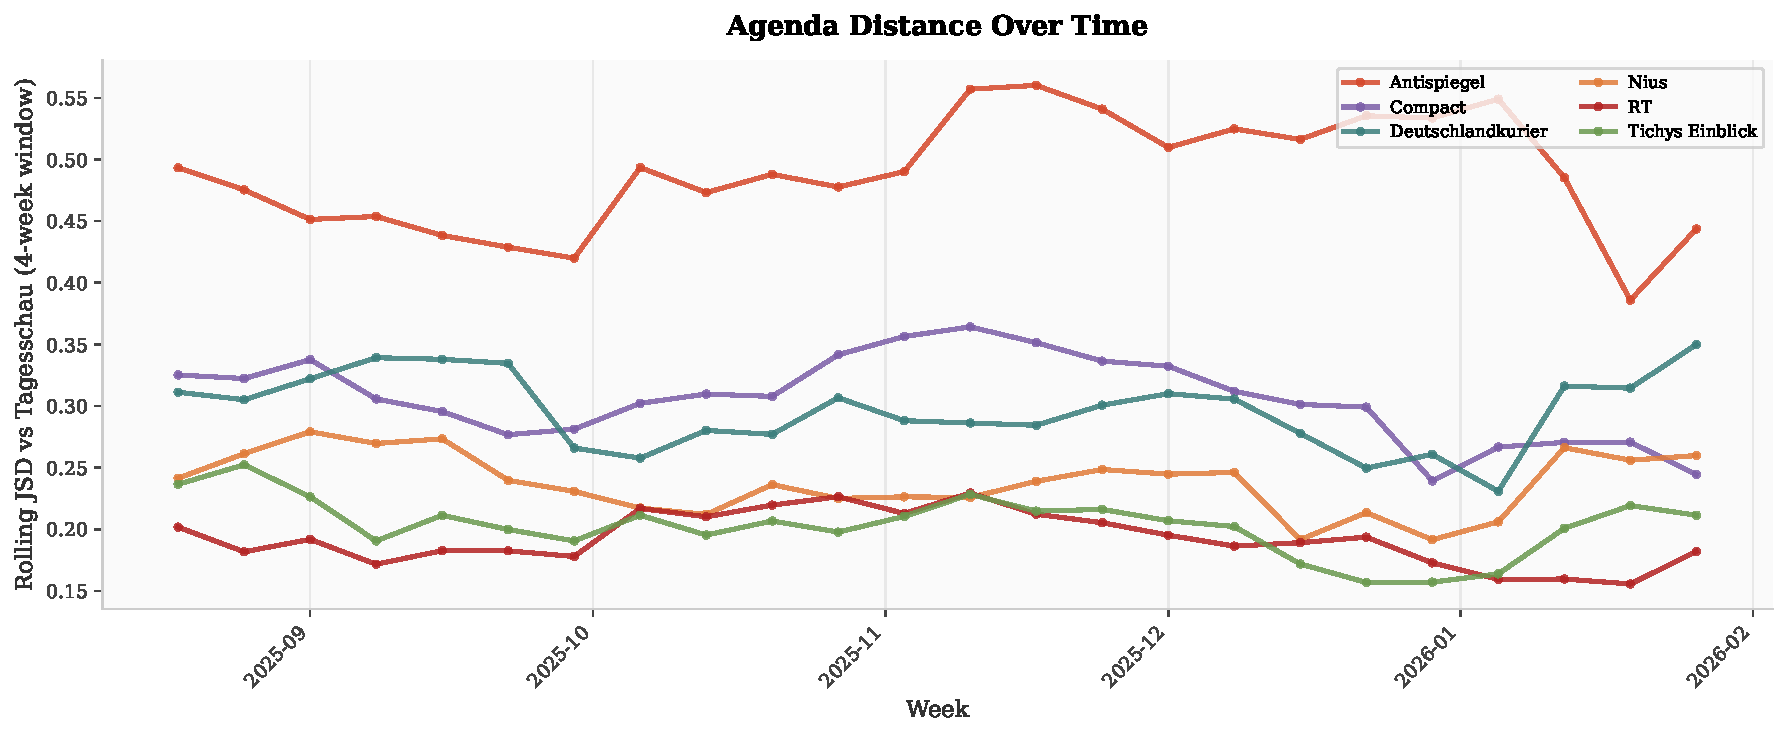
\includegraphics[width=\textwidth]{Images/h1/h1_11_rolling_jsd.pdf}
    \caption{Rolling JSD vs Tagesschau (4-week sliding window). Agenda distance is structurally stable for all outlets, with low variance and no systematic trend. Anti-Spiegel maintains consistently the highest distance throughout the study period.}
    \label{fig:h1_rolling_jsd}
\end{figure}

Figure~\ref{fig:h1_rolling_jsd} shows that agenda distance is remarkably stable over time. Coefficients of variation (standard deviation divided by mean) range from 0.09 to 0.11 across all outlets, indicating that the observed distortion is a structural property of each outlet's editorial strategy rather than a transient response to specific news events. No outlet shows a systematic trend toward convergence with or divergence from the mainstream agenda during the study period.

Time-lagged cross-correlations for key topics (AfD/parties, Ukraine/Putin, migration) show that coverage peaks are predominantly simultaneous across outlets (peak at lag = 0), suggesting that both mainstream and alternative outlets react to the same external events. The distortion manifests not in \textit{when} topics are covered but in \textit{how much} emphasis they receive---a persistent amplification rather than a temporal lead or lag.

\subsection{Robustness}

To ensure that findings are not artifacts of modelling choices, corpus size imbalance, or statistical chance, we conducted nine robustness checks. Table~\ref{tab:robustness} summarises the results.

\begin{table}[H]
\centering
\caption{Summary of robustness checks for H1 findings}
\label{tab:robustness}
\begin{tabular}{llp{7.5cm}}
\hline
\textbf{\#} & \textbf{Check} & \textbf{Result} \\
\hline
1 & Permutation test ($n = 500$) & All $p = 0.000$; observed JSD 14--50$\times$ above null mean \\
2 & Bootstrap CIs ($n = 500$) & All JSD and Spearman CIs exclude null values \\
3 & Downsampling ($n = 50$, 565 articles) & Rankings preserved at equal corpus sizes \\
4 & Merge threshold sensitivity & Rankings stable across min\_similarity 0.5--0.7 \\
5 & Outlier reduction impact & Metrics near-identical with and without reduction \\
6 & Outlet clustering & Clusters match a priori ideological categories \\
7 & Per-topic $\chi^2$ tests & 275/444 significant at FDR $< 0.01$ \\
8 & Global model validation & JSD ranking $\rho = 0.943$ vs merged model \\
9 & Temporal stability & Stable rolling JSD (CV = 0.09--0.11) \\
\hline
\end{tabular}
\end{table}

The permutation test (check 1) shuffled outlet labels while keeping topic assignments fixed, establishing that observed JSD values are 14--50 times larger than what would be expected under random outlet assignment. The downsampling test (check 3) equalised all outlets to the size of the smallest corpus (Anti-Spiegel, $n = 565$) across 50 resamples, demonstrating that distortion rankings are preserved when size imbalance is eliminated. The sensitivity analysis (check 4) re-merged per-outlet models at similarity thresholds of 0.5, 0.6, 0.7, and 0.8, finding stable rankings across 0.5--0.7 with minor instability only at 0.8 (where 114 topics may be too granular). All nine checks pass, confirming that H1 findings are robust to modelling decisions, corpus characteristics, and statistical assumptions.

\subsection{Summary of Findings}

\textbf{Hypothesis 1 is supported.} All six alternative outlets exhibit statistically significant and robust agenda distortion compared to the Tagesschau mainstream reference. The distortion manifests in two complementary patterns:

\begin{enumerate}
    \item \textbf{Agenda amplification}: Right-wing and right-populist outlets systematically amplify domestic political conflict topics---party politics (+5.5pp), the chancellor race (+4.7pp), social media discourse (+4.0pp), and migration (+2.2pp)---while de-prioritising apolitical coverage such as financial markets and international non-conflict news.

    \item \textbf{Agenda substitution}: Pro-Russian outlets substitute large portions of their agenda with Russia/Ukraine coverage from a Russian perspective, accounting for 32\% (RT DE) to 49\% (Anti-Spiegel) of their content versus 9\% for Tagesschau.
\end{enumerate}

The distortion gradient follows outlet categories: strongest among pro-Russian outlets (Anti-Spiegel JSD = 0.40), moderate among right-wing outlets (Deutschland-Kurier JSD = 0.22, Compact JSD = 0.21), and mildest among right-populist outlets (NIUS JSD = 0.19, Tichys Einblick JSD = 0.15). This gradient is temporally stable, empirically validated through outlet clustering, and robust across nine independent checks.
